%!TEX root=main.tex
\subsection{Specifications}
The goal of this project is to design and simulate a delay measurement device using components available through the AMS C35 \SI{0.35}{\micro\meter} CMOS process.
In order to measure the length of a long cable, a voltage pulse is applied to one end of the cable and the length is deduced from the time it takes to reach the other end.

The output of the device must scale with the delay between two voltage pulses, which can range between \SI{10}{\nano\second} and \SI{500}{\nano\second}.
The pulses themselves are chosen to be \SI{10}{\nano\second} long, and the device must be able to drive a \SI{10}{\pico\farad} capacitive load.

\subsection{Basic Block Diagram}
To achieve this, the device is organized as shown in figure~\ref{fig:block}.
\begin{figure}
  \centering
  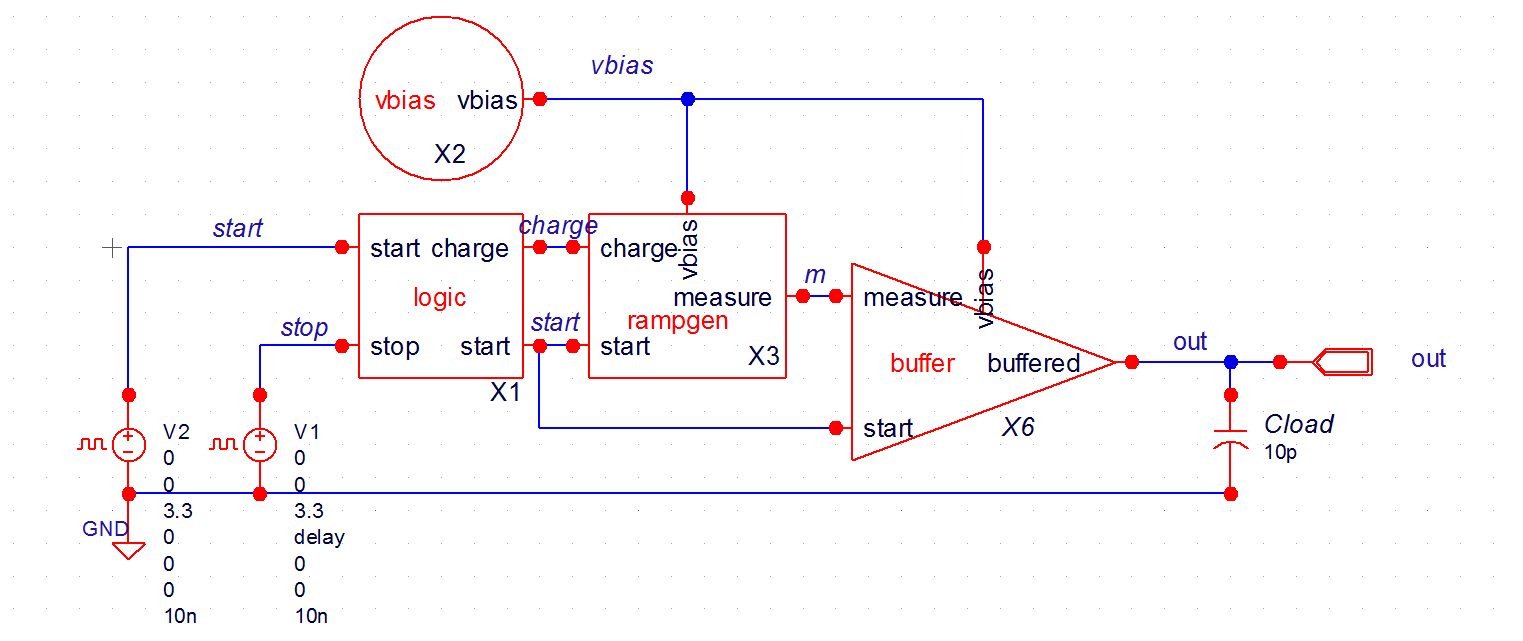
\includegraphics[width=\textwidth]{blocks.png}
  \caption{Block diagram overview of the delay measurement device.\label{fig:block}}
\end{figure}

At the core is the block \blk{rampgen} which generates a rising ramp on its analog output \sig{measure} when the digital input \sig{charge} is \sigval{LO}, maintains its output when \sig{charge} is \sigval{HI}, and resets it to ground when the digital input \sig{start} is \sigval{HI}.

It is the controlled by the first block, \blk{logic}, which controls its digital outputs \sig{charge} and \sig{start}\footnote{The fact that the output has the same name as the input can be confusing. As presented in the next section, in our implementation we end up with $\sig{start}_{out}$ = $\sig{start}_{in}$ and unfortunately Gateway then forces us to use the same name for the signal, even if we had rather named it \sig{reset} at the output of \blk{logic}. In the remain of this report, this will be clarified using subscripts when necessary.} based on the succession of pulses on its digital inputs \sig{start} and \sig{stop} and some internal logic.

The output of \blk{rampgen} is buffered by the output stage \blk{buffer} which is able to drive the specified load of \SI{10}{\pico\farad}.

In the next three sections, the design of each of these blocks is reviewed. Then, in section \ref{sec:bias}, some biasing considerations are presented. Finally, in the last section, the operation curves of the device are presented.
